\subsection{Lizenzen}\label{sec:lizenzen}
Die Lizenztexte sind alle in Englisch veröffentlicht. Dadurch kann das Projektteam nicht haftbar gemacht werden für unwissentlich gemachte Übersetzungsfehler.

\subsubsection*{SDK}
Nordic Semiconductor hat an Anfang eines jeden Files ihren Lizenztext \cite{nordic_sdk_license} hinterlegt. In diesem ist Beschrieben was mit dem Code gemacht werden darf und was nicht. Einige wichtige Punkte:

\begin{itemize}
	\item Am Anfang jedes Files muss der Lizenztext stehen.
	\item Weiterverteilung muss unter dem Selben Copyright erfolgen wie bisher.
	\item Mann soll nicht ungefragt Werbung machen für Nordic und Co.
	\item Die Software darf nur für NRF-Chips verwendet werden.
\end{itemize}

Auch werden alle Verantwortungen für Support, Sicherheit usw. abgestritten. Damit sind sie nicht Haftbar für Schäden, die die Software anrichtet.

Der S132 ist speziell, weil dieser nicht in Source-Form vorliegt. Er ist nur in Binary-Form enthalten. Er hat einen leicht anderen Lizenztext welcher in der SDK neben den Biarys gefunden werden kann. Er besagt zusätzlich, dass der Sourcecode der Softdevice nicht reverse engineered, decompilert, modifiziert und disassembliert werden darf.

\subsubsection{FatFs}
Die FatFs Library untersteht einer 1-clause BSD Lizenz. Dies bedeutet sie darf verwendet werden, muss aber den Lizenztext aus Abbildung \ref{fig Lizenztext FatFs}.


\begin{figure}[ht!]
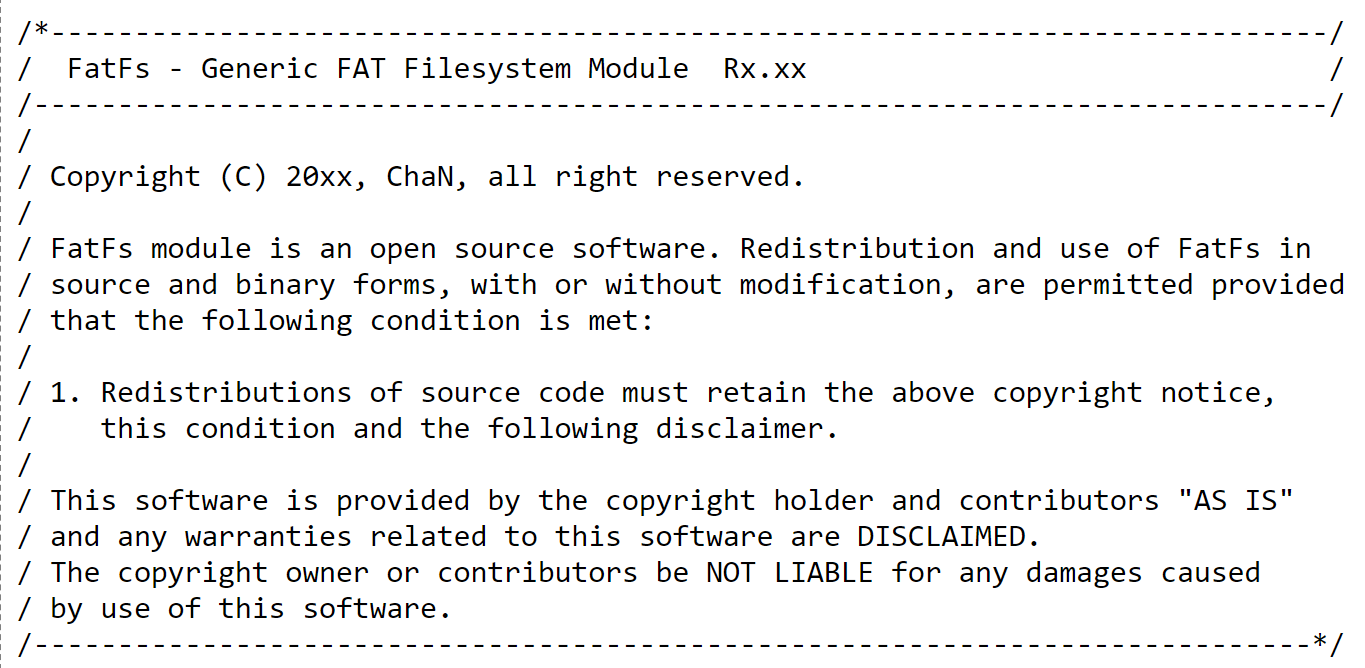
\includegraphics[width = 140mm]{data/Lizenztext_FatFs.png}
\caption{Lizenztext FatFs Library}
\label{fig Lizenztext FatFs}
\end{figure}
